\documentclass[10pt]{beamer}
\usetheme[
%%% option passed to the outer theme
% progressstyle=fixedCircCnt,   % fixedCircCnt, movingCircCnt (moving is deault)
]{Feather}

% If you want to change the colors of the various elements in the theme, edit and uncomment the following lines

% Change the bar colors:
% \setbeamercolor{Feather}{fg=red!20,bg=red}

% Change the color of the structural elements:
% \setbeamercolor{structure}{fg=red}

% Change the frame title text color:
% \setbeamercolor{frametitle}{fg=blue}

% Change the normal text color background:
% \setbeamercolor{normal text}{fg=black,bg=gray!10}

% -------------------------------------------------------
% INCLUDE PACKAGES
% -------------------------------------------------------

\usepackage[utf8]{inputenc}
\usepackage[italian]{babel}
\usepackage[T1]{fontenc}
\usepackage{helvet}
\usepackage{pgfplots}
\usepackage{ragged2e}
\usepackage{ocg-p}
\usepackage{blindtext}
\usepackage{hyperref}
\usepackage{pgfplots, pgfplotstable}
\usepackage{siunitx}
\usepackage{placeins}
\usepackage{datetime}
\usepackage{animate}
\usepackage{tikz}
\usepackage{graphics}
\newdate{date}{21}{12}{2017}

% -------------------------------------------------------
% DEFFINING AND REDEFINING COMMANDS
% -------------------------------------------------------

% colored hyperlinks
\newcommand{\chref}[2]{
  \href{#1}{{\usebeamercolor[bg]{Feather}#2}}
}

% -------------------------------------------------------
% INFORMATION IN THE TITLE PAGE
% -------------------------------------------------------
% \setbeamertemplate{title page}
% {
\title[Tesi di laurea magistrale Simone Massenzio ] % [] is optional - is placed on the bottom of the
% sidebar on every slide
{ Confronto fra le caratteristiche
  fisico-strutturali di suoli in area
  Mediterranea sottoposti a diversi metodi di
  conduzione e lavorazione}


% \subtitle[Uno studio di fisica del suolo]{
% Uno studio di fisica del suolo
% }

\author[Simone Massenzio]{ 
  Candidato: Simone Massenzio \\
  Relatore: Dott. O.L. Pantani\\
  \vspace{0.1cm}
  Correlatori:
  Dott. L.P. D'Acqui, Prof. G.C. Pacini}     



\institute[] { \emph{Dipartimento di Scienze della Produzioni Animali e
    dell'Ambiente\\
    Universit\`a degli studi di Firenze - UniFI\\}
  
  % there must be an empty line above this line - otherwise some
  % unwanted space is added between the university and the country (I
  %   % do not know why;( )
}

\date{\displaydate{date}}


% -------------------------------------------------------
% THE BODY OF THE PRESENTATION
% -------------------------------------------------------
\setbeamercovered{transparent}


\begin{document}
{\1
  \begin{frame}[noframenumbering]%{\footnotesize{Dipartimento di Scienze della Produzioni Animali e
    % dell'Ambiente\\
    % Universit\`a degli studi di Firenze - UniFI}}
    \titlepage
  \end{frame}}


% presumo che queste righe mettano dei segnali in ogni parte e sezione
% \AtBeginPart{\frame<beamer>{\partpage
% \transsplitverticalout[duration=1] 
% \begin{block}{}
%       %   \tableofcontents[subsectionstyle=show]
%   \tableofcontents[subsectionstyle=hide]
% \end{block}
% }}

%   \AtBeginSection[]{\frame<beamer>{%
%   \begin{block}{}
%     \tableofcontents[currentsection, subsectionstyle=hide]
%   \end{block}
% }
% }




\begin{frame}{Obiettivi}{}
  %\transdissolve<1>
  %\transdissolve<2>
  \begin{columns}[c]
    \column{.50\textwidth}
    \begin{itemize}[<+->]
      \pause
    \item verificare la presenza di differenze nelle caratteristiche
      fisiche del suolo in aree: coltivate convenzionalmente oppure
      coltivate a biologico tramite indicatori fisici di fertilità del
      suolo
    \item verificare eventuali effetti dovuti a diverse lavorazioni
      (aratura, rippatura, frangizollatura).
    \end{itemize}
    \column{.48\textwidth}
    \only<2>{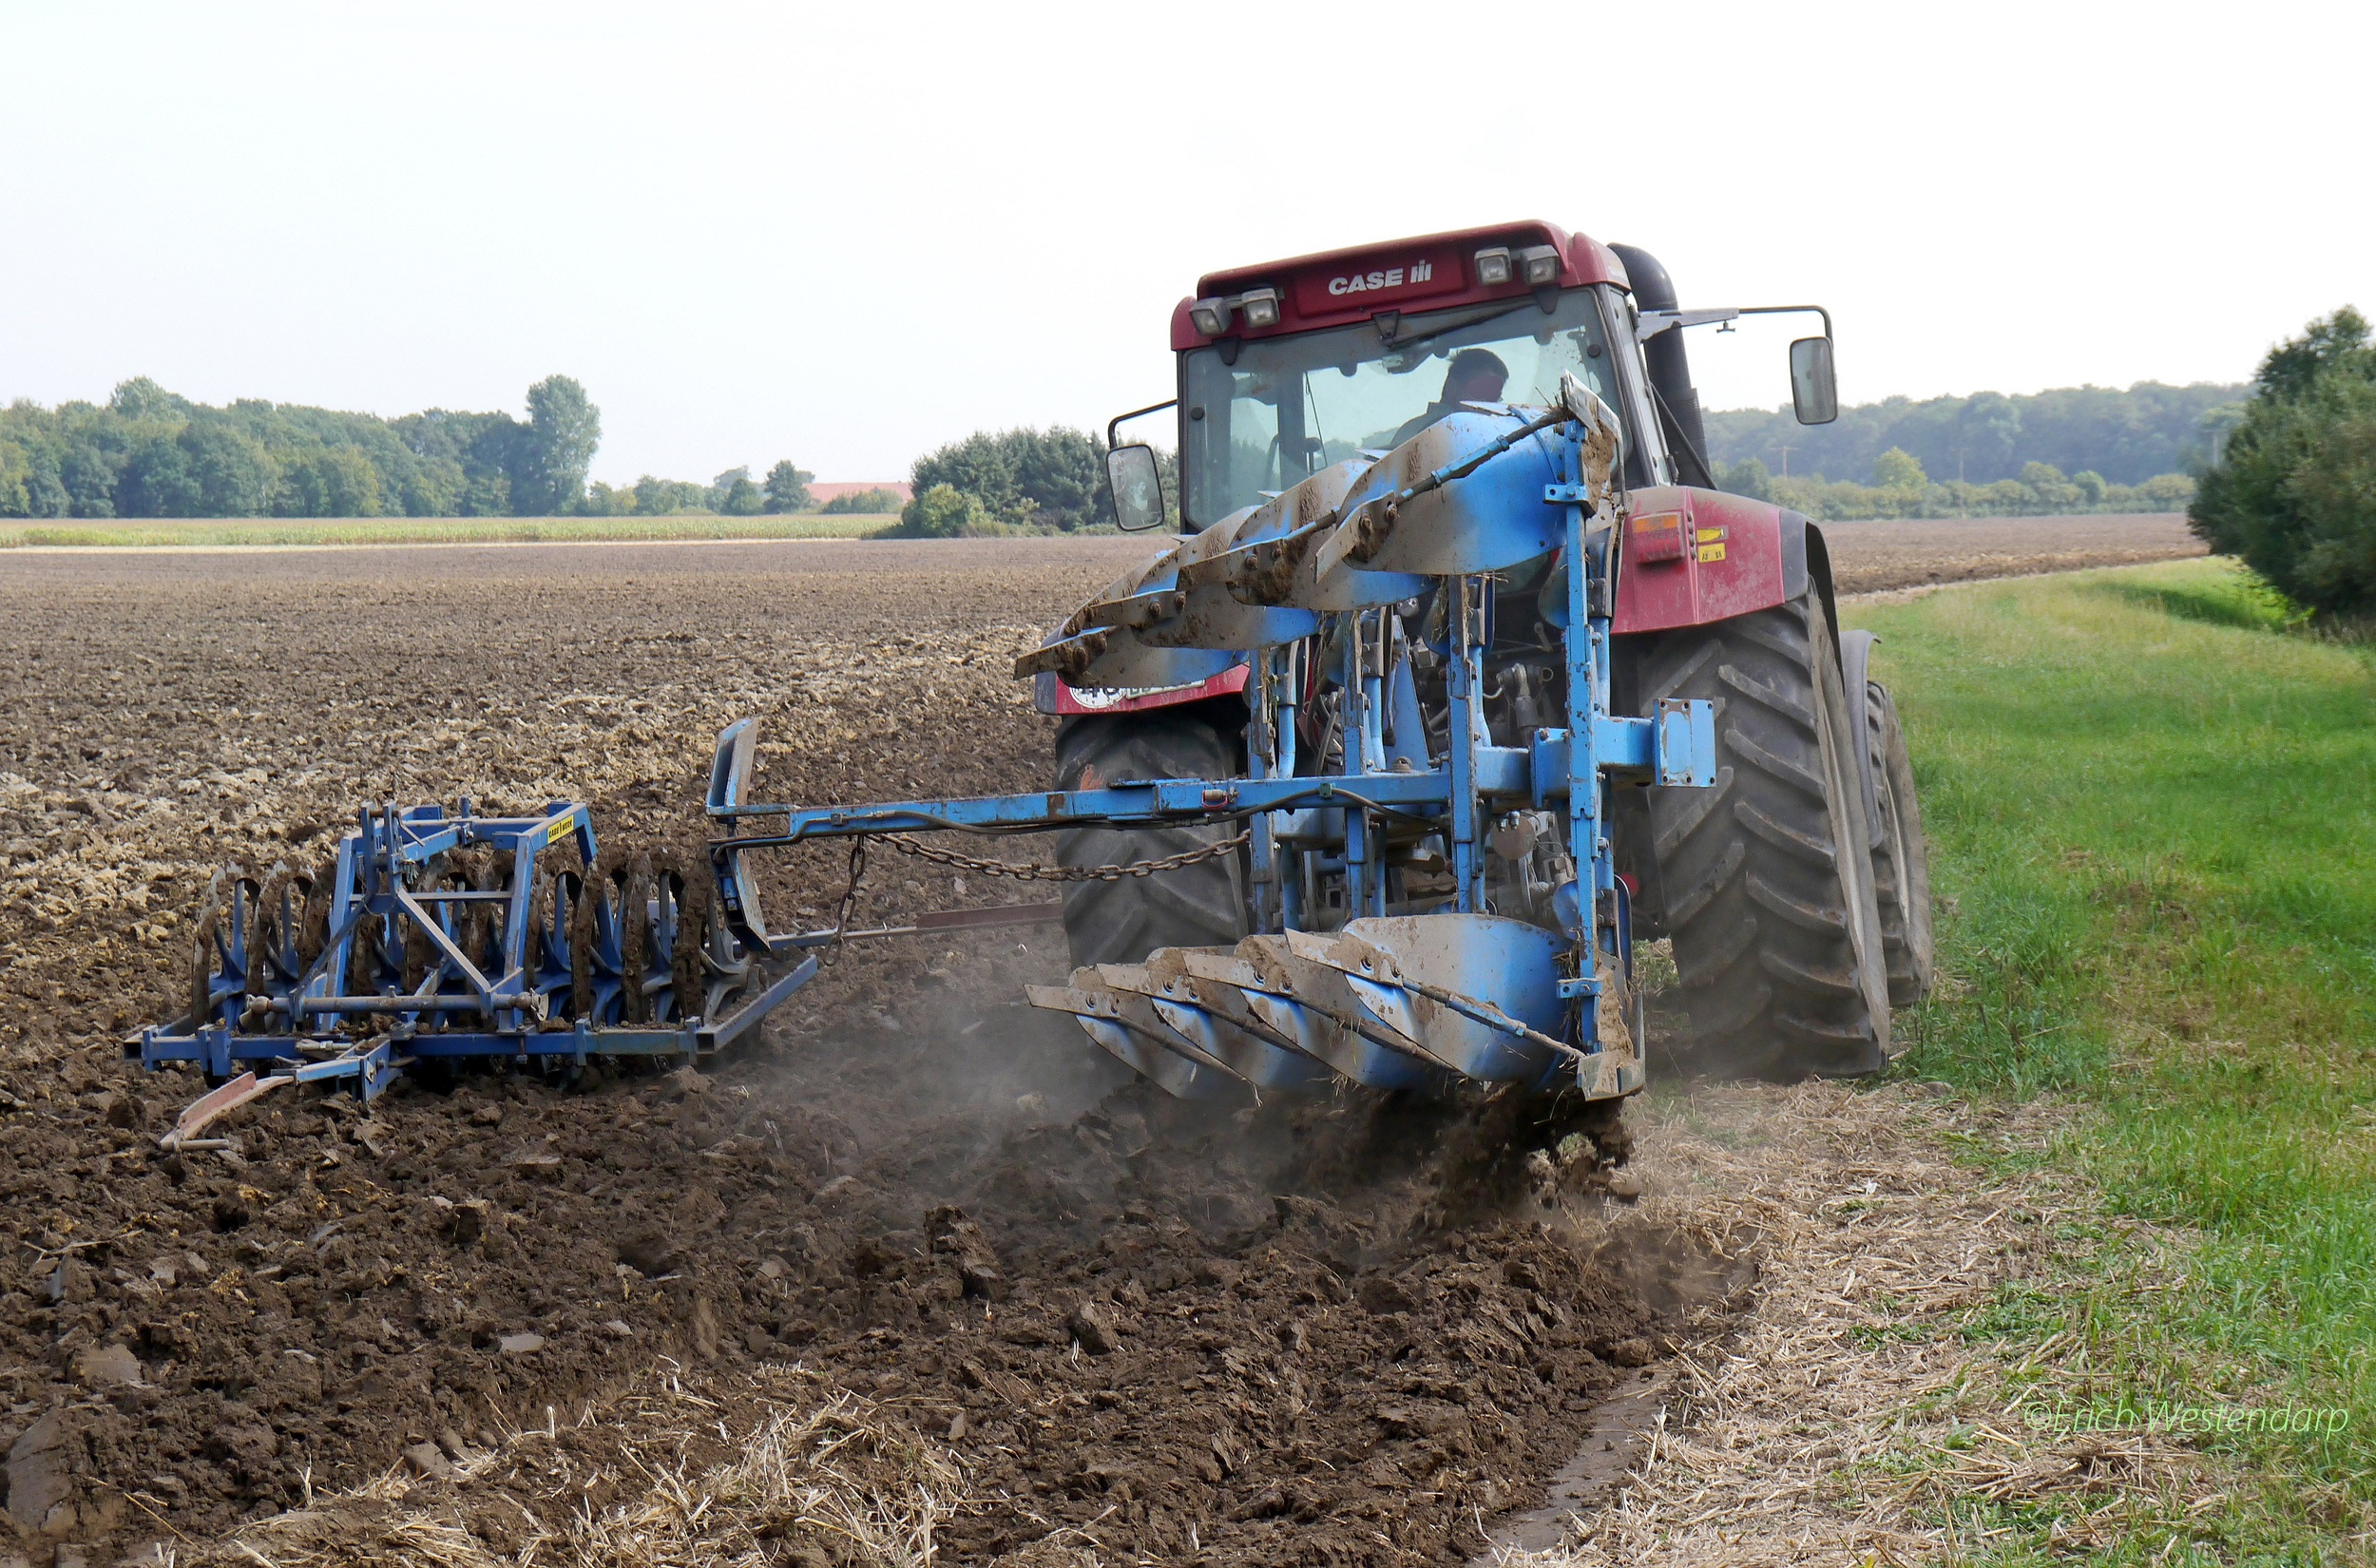
\includegraphics[width=0.8\textwidth]{../foto/lavorazione.jpg}}
    \only<3>{\includegraphics[width=0.8\textwidth]{../foto/logo-Bio.png}}
  \end{columns}
\end{frame}

\begin{frame}
  \begin{columns}[c]
    \column{.50\textwidth}
    \begin{itemize}[<+->]
    \item Densit\`a apparente
      \begin{itemize}
      \item Metodo \emph{Core}
      \pause
      \item Metodo \emph{Clod}
      \pause
      \end{itemize}
    \item Stabilit\`a degli aggregati tramite dinamica della
      distribuzione della dimensione degli aggregati;
    \item Distribuzione dimensionale dei pori tramite tecniche di
      porosimetria ad intrusione di mercurio;      
    \end{itemize}
    \column{.48\textwidth}
    \begin{overlayarea}{\linewidth}{3cm}
      \only<2>{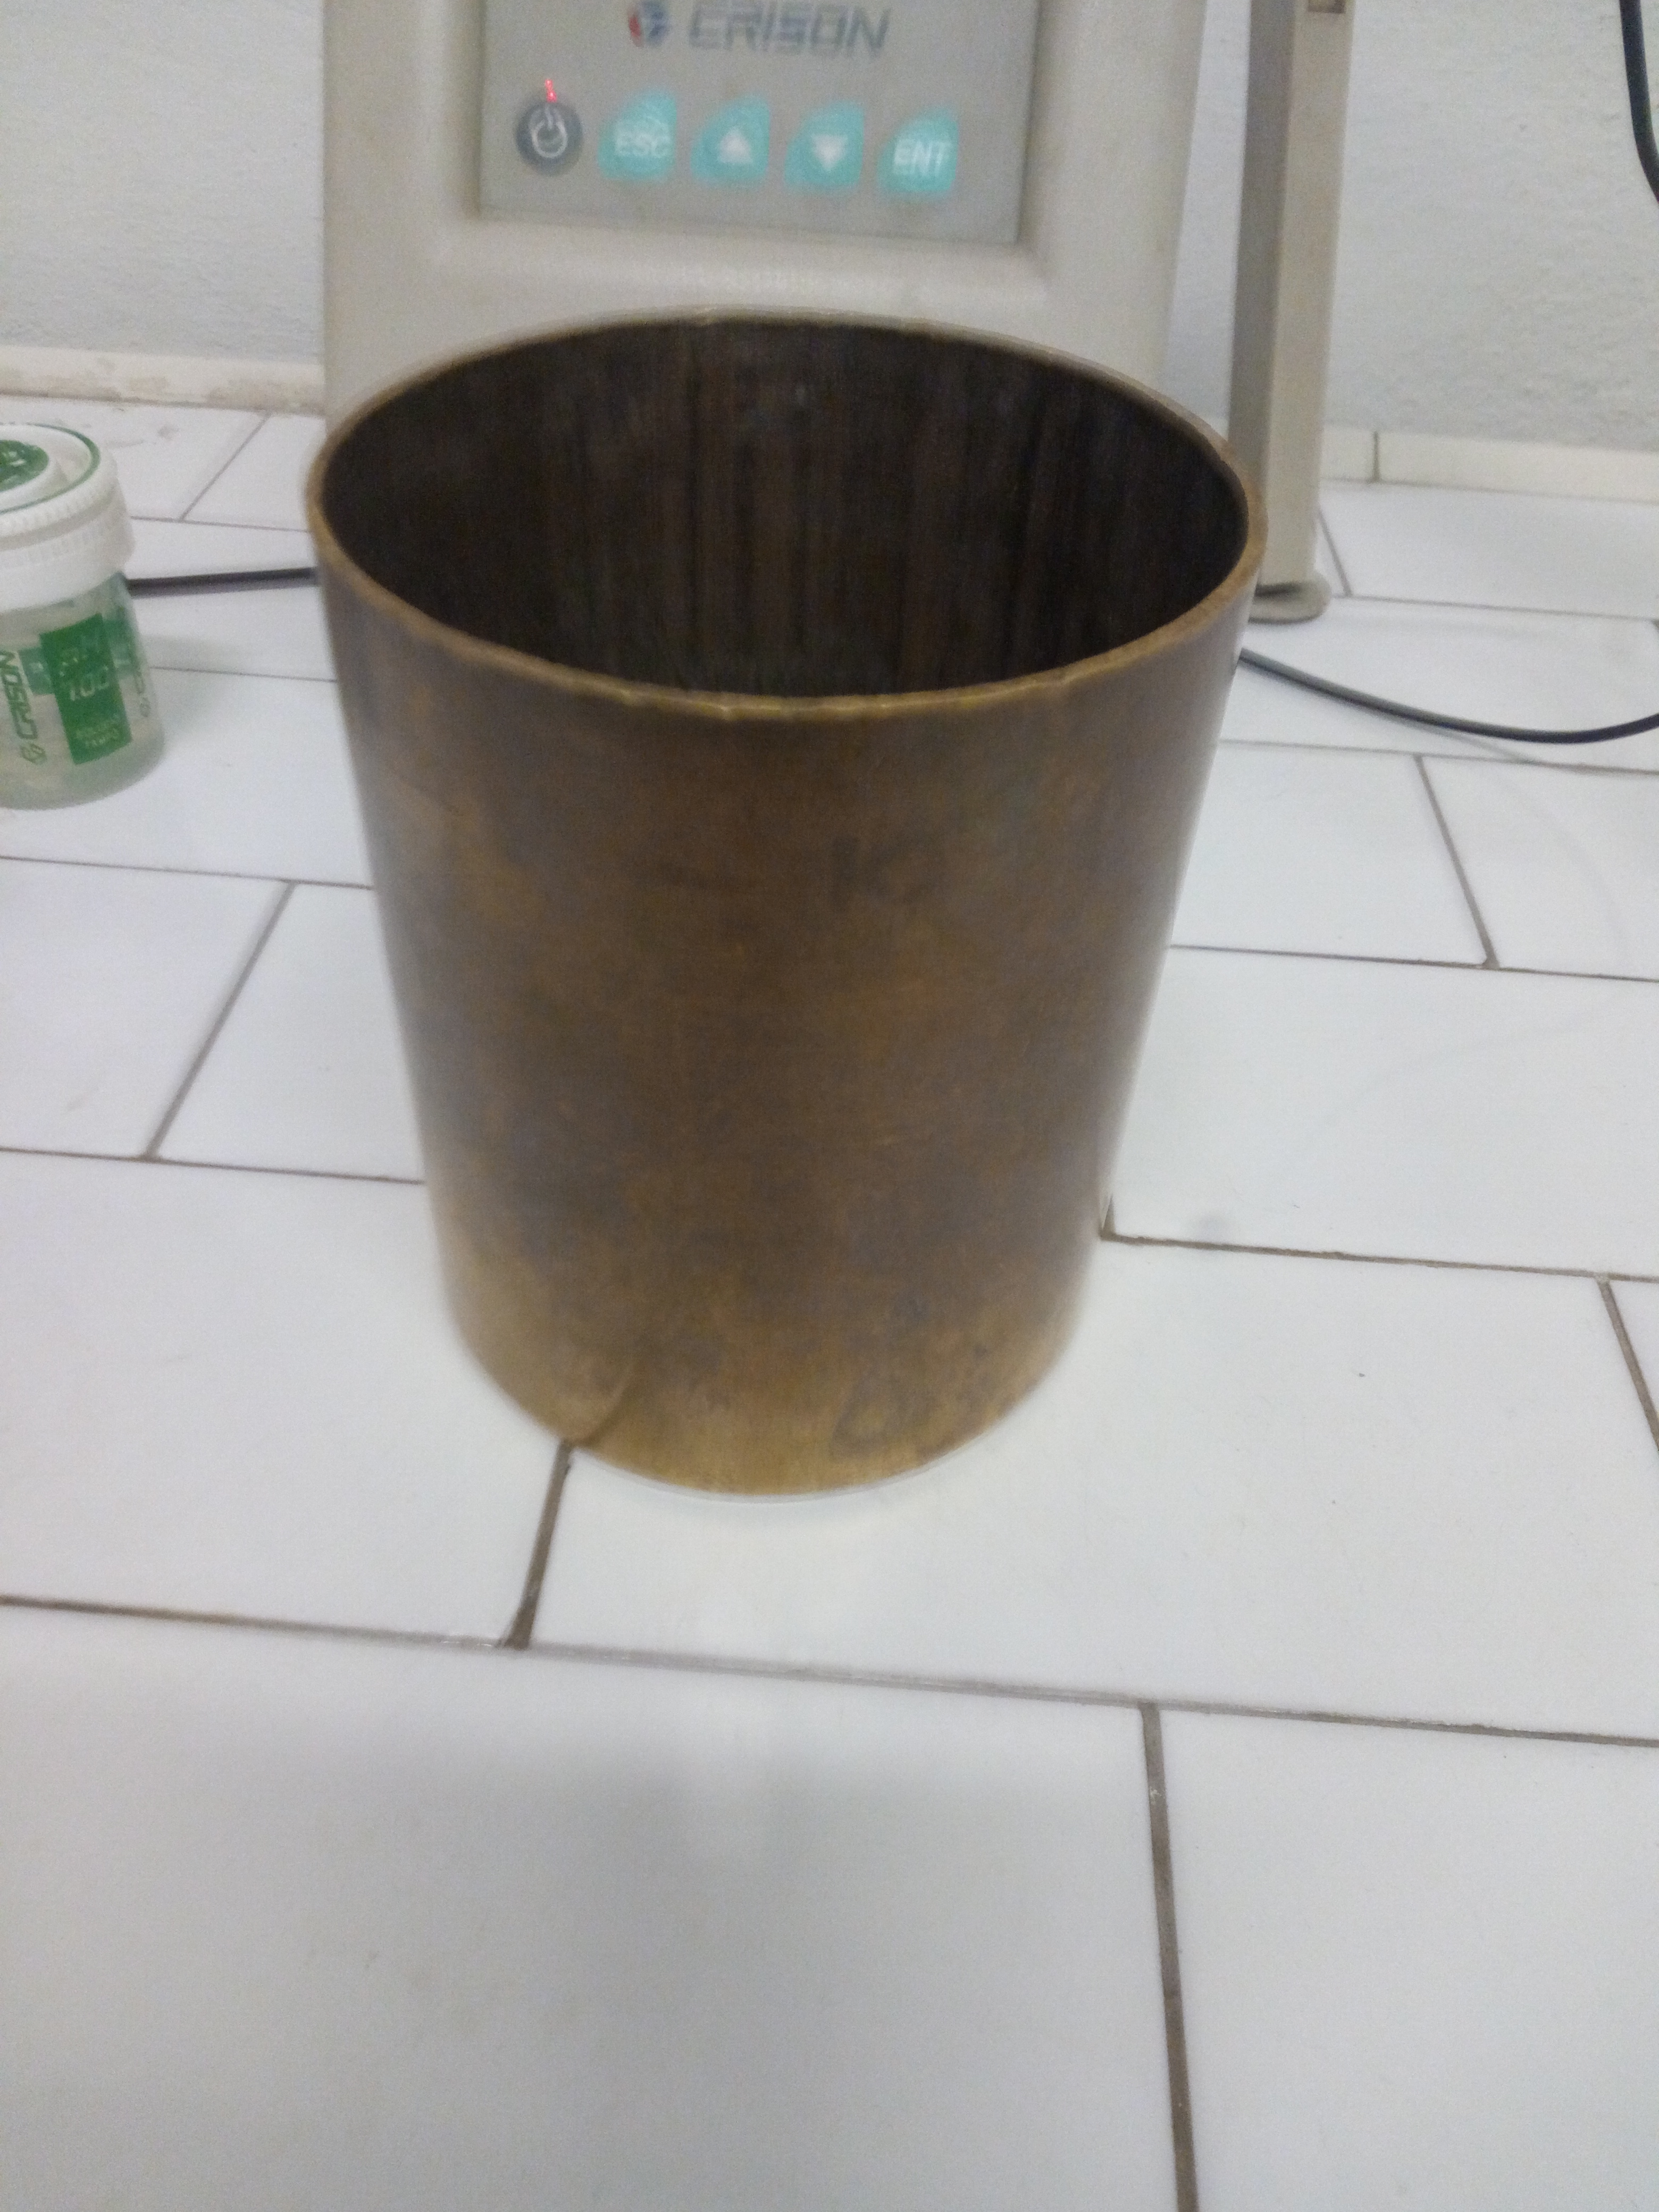
\includegraphics[width=0.8\textwidth]{../foto/cilindroOttone.jpeg}}
      \only<3>{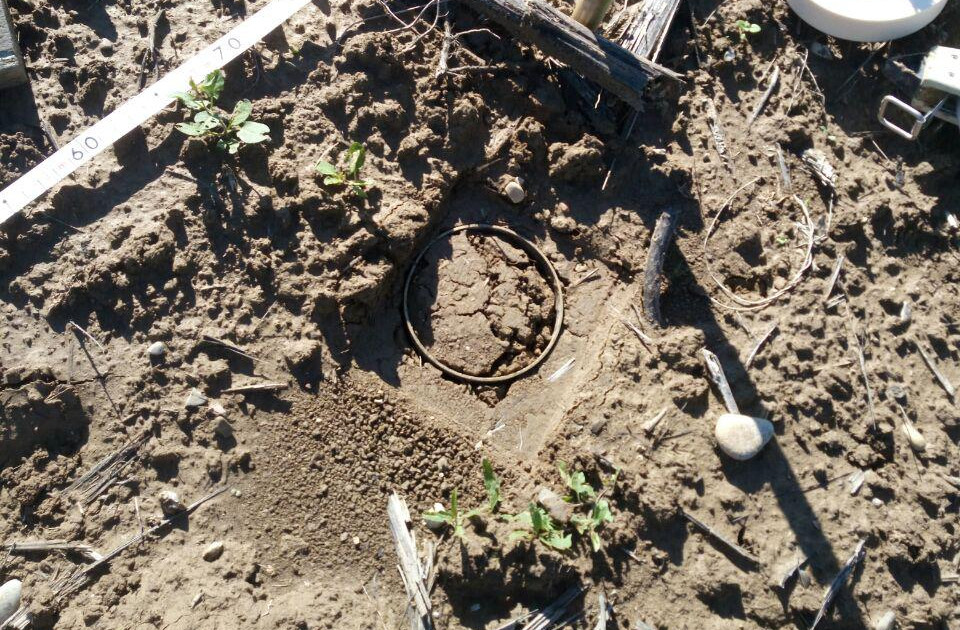
\includegraphics[width=0.8\textwidth]{../foto/cilindrosuolo.jpg}}
      \only<4>{\vspace{1cm}
\begin{figure}[hb]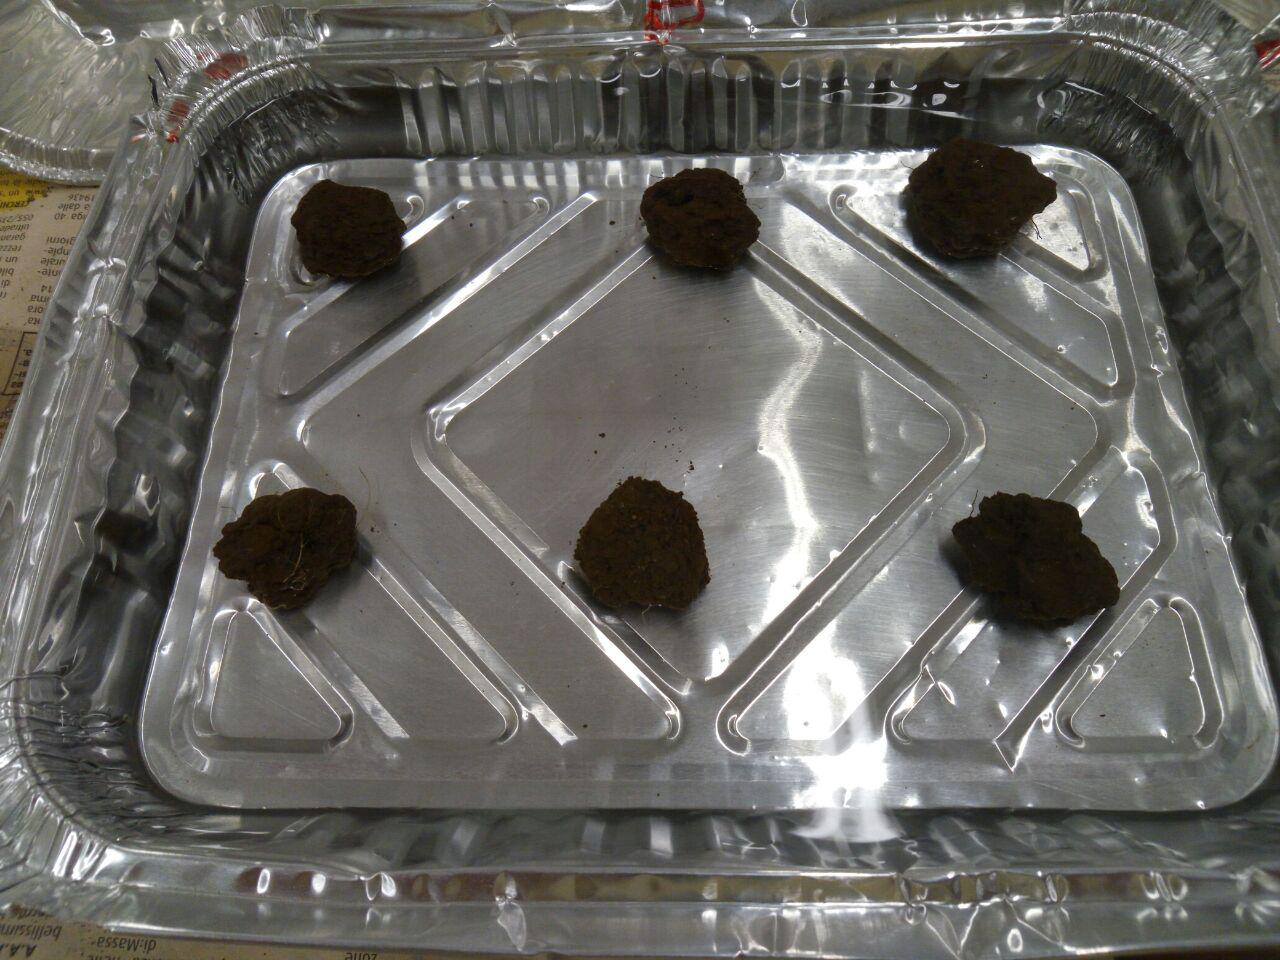
\includegraphics[width=0.8\textwidth]{../foto/petrolio}
\end{figure}}
      \only<5>{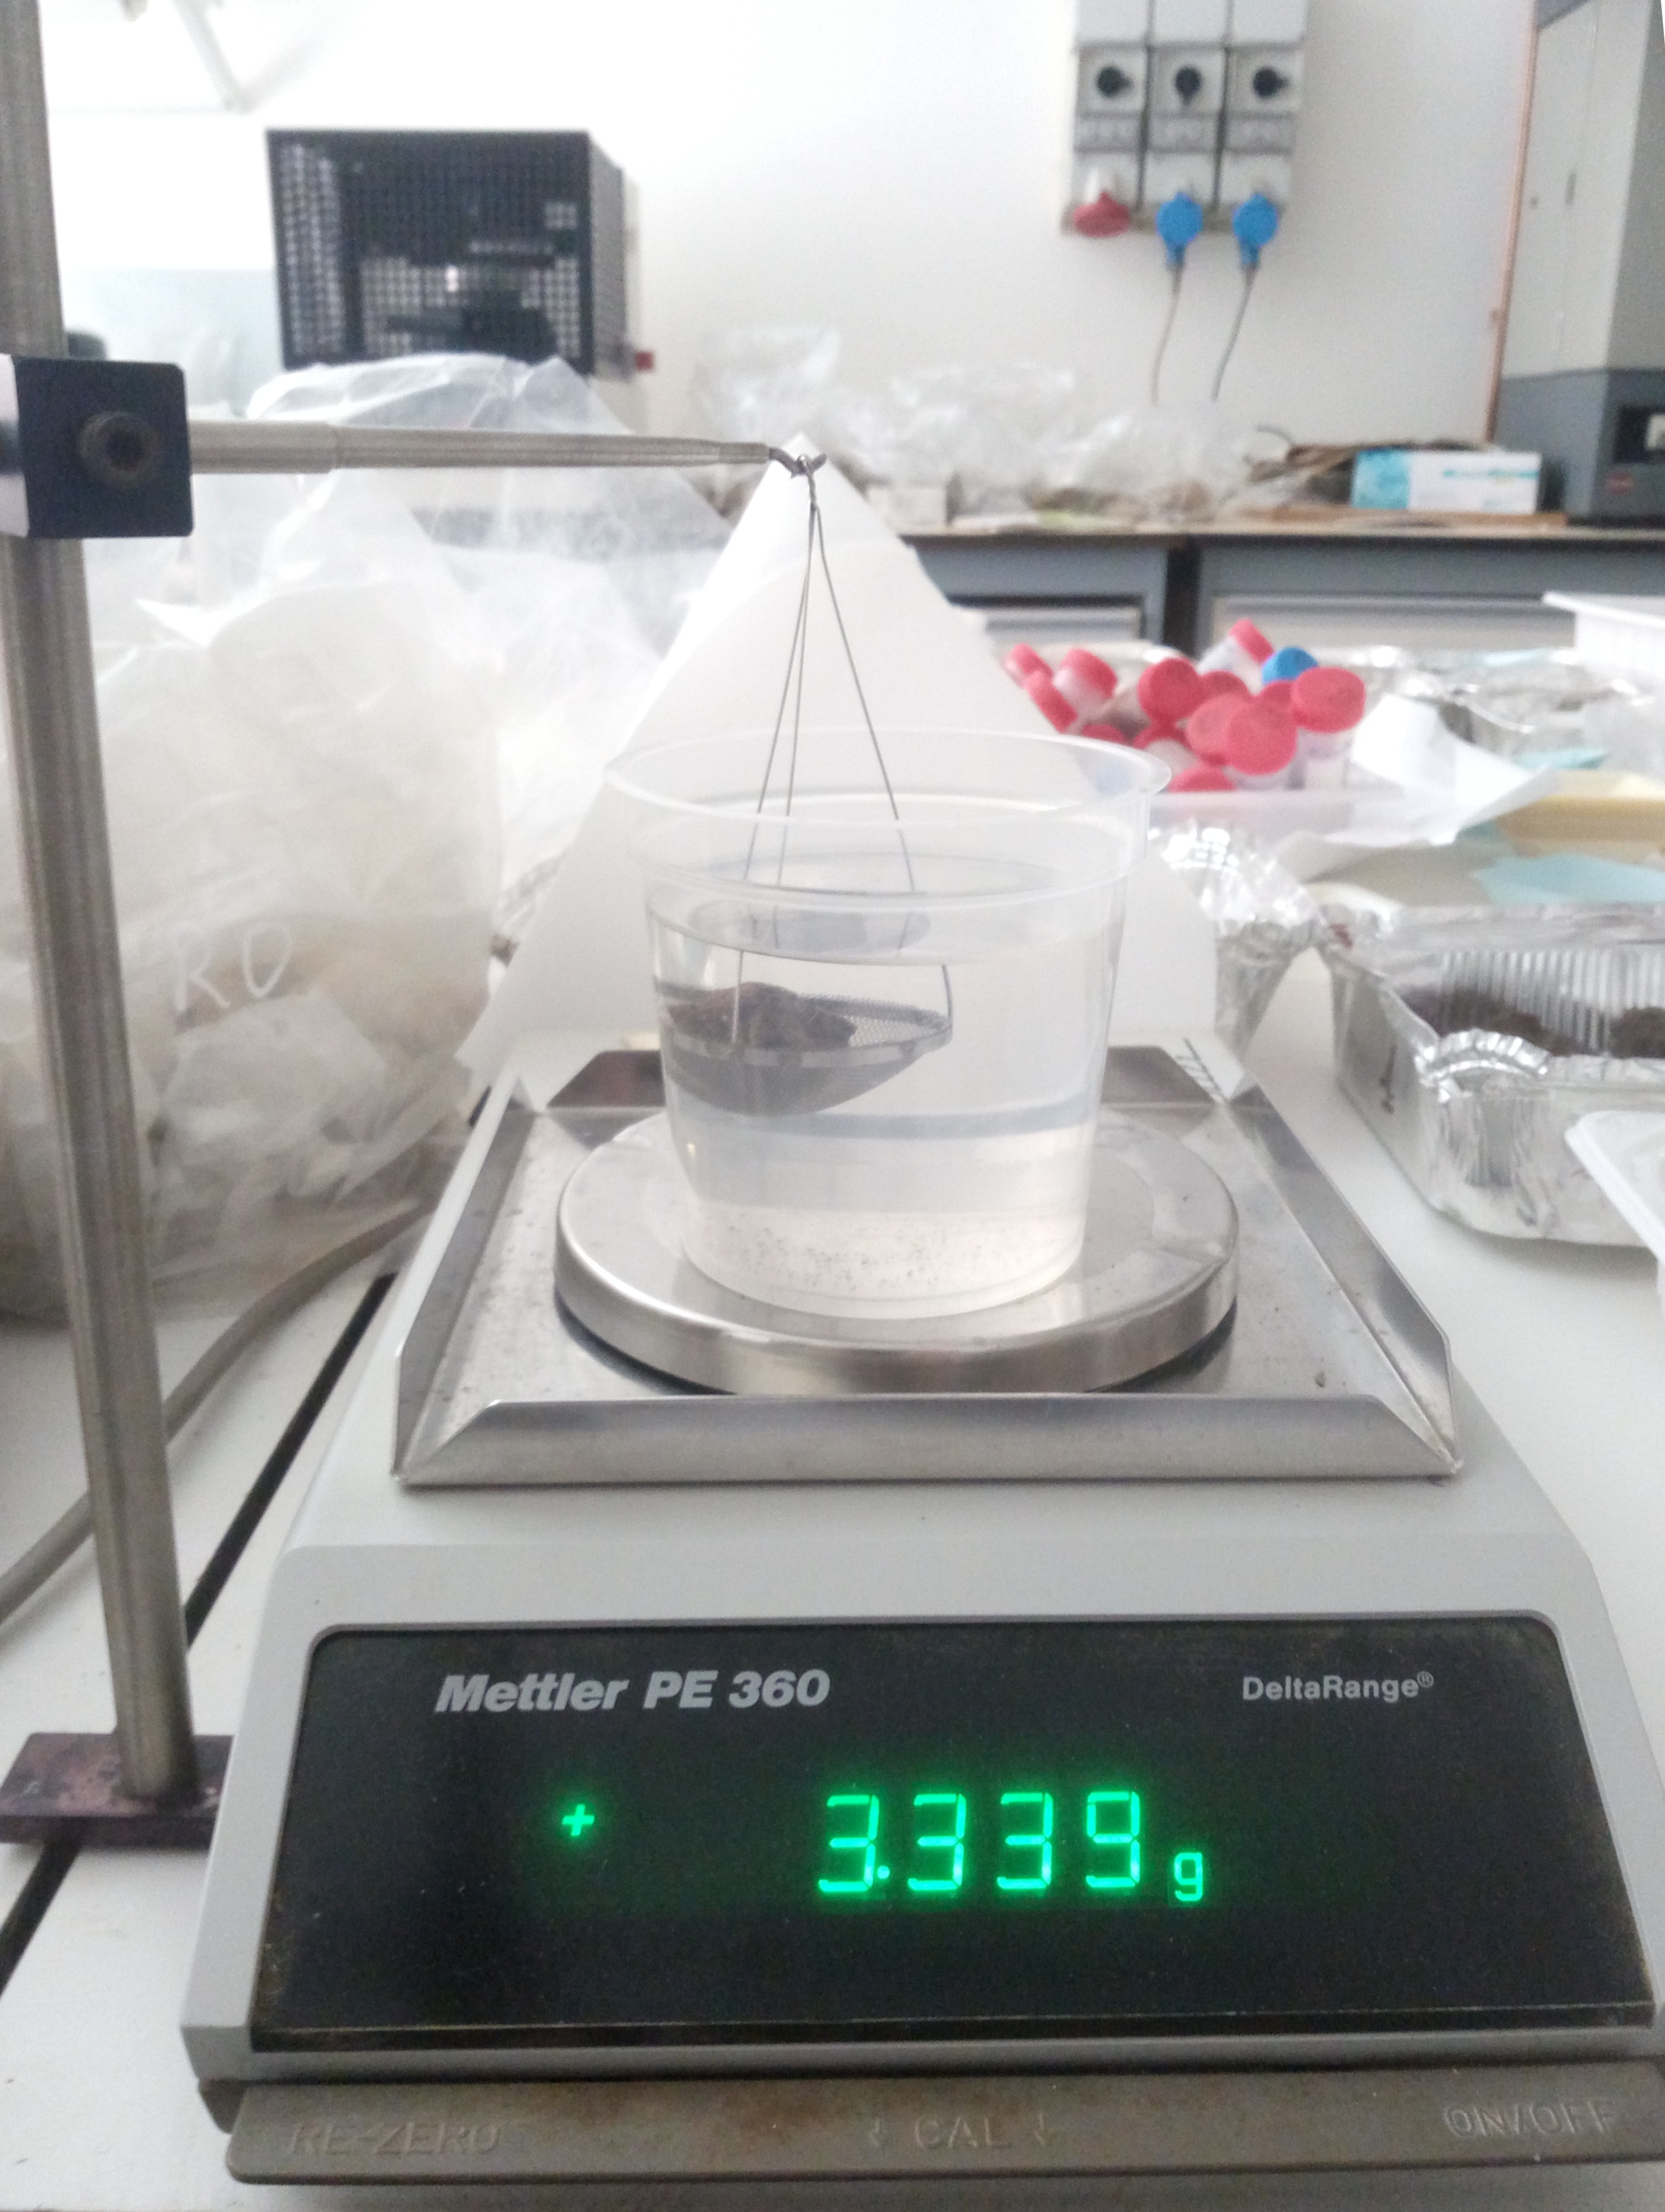
\includegraphics[width=0.8\textwidth]{../foto/navicella}}
      \only<6>{\animategraphics[loop,autoplay,width=\linewidth]{12}{../foto/msizer/Msizer-}{0}{2}}%233
      \only<7>{\animategraphics[loop,autoplay,width=\linewidth]{12}{../foto/poresize/PoreSize-}{0}{2}}%%396
    \end{overlayarea}
  \end{columns}
\end{frame}



\begin{frame}
  \frametitle{Analisi statistica}
  \transwipe<4>[direction=90]
  L'elaborazione dei dati è stata effettuata mediante il linguaggio di
  programmazione R, ed ha riguardato:
  \begin{itemize}
    \onslide<2->\item la costruzione di un modello lineare nella forma:
    \vspace{0.25cm}
    $Y \sim \mu + \beta_1x_1 + \beta_2x_2 + \epsilon$

    \onslide<3->{in cui le variabili categoriche sono:}
    \begin{itemize}

      \onslide<4->\item $\beta_1$ conduzione \newline
      \emph{Convenzionale}, \emph{Biologico}

      \onslide<5->\item $\beta_2$ lavorazioni \newline \emph{Arato, Rippato,
        Frangizollato}

      \onslide<6->\item$\epsilon$ residui o errore
    \end{itemize}
    \onslide<7->\item la validazione del modello attraverso l'analisi
    dei residui 
    \onslide<8->\item verifica della significatività delle ipotesi mediante analisi della varianza (ANOVA)
  \end{itemize}
\end{frame}


\begin{frame}

  \begin{columns}
    \column{.50\textwidth}
    \vspace{1cm}
    \footnotesize
    \begin{itemize}[<+->]
    \item I dati ottenuti dalle analisi di porosimetria e
      stabilità degli aggregati sono delle distribuzioni in cui ogni
      classe dimensionale è espressa come percentuale sul volume totale,
      questo tipo di dati prende il nome di \emph{dati Composizionali}
      \pause
    \item Per rappresentare i dati composizionali si utilizza un
      grafico triangolare. Per l'elaborazione è necessaria
      un'operazione di linearizzazione
    \item Queste operazioni sono state effettuate tramite il package 'composition' del
      linguaggio di programmazione R
    \end{itemize}

    \column{.48\textwidth}
    \only<2>{\begin{overlayarea}{\linewidth}{3cm}
        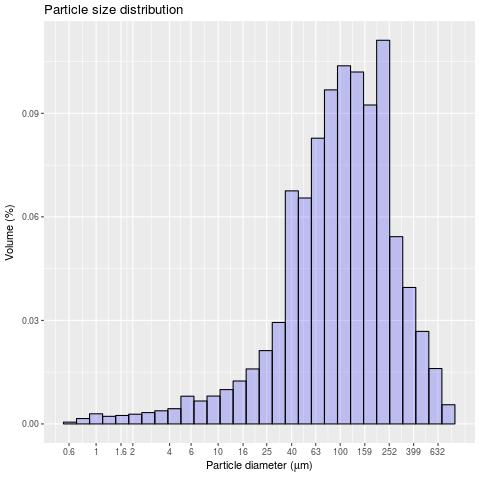
\includegraphics[width=\textwidth]{../grafici/boh.jpeg}
      \end{overlayarea}}
    \only<3>{\begin{overlayarea}{\linewidth}{2cm}\includegraphics[width=\textwidth]{../foto/simplessodeforma.png}     
      \end{overlayarea}}
  \end{columns}
\end{frame}

% \begin{frame}[label=Composizionale]
%   \vspace{2cm}
%   Risultati analisi \hyperlink{Anova}{\beamerbutton{composizionale}}
%   \begin{figure}[hb]
%     \includegraphics[width=0.6\textwidth]{../tesi/Tesi_GIT-plotacompWETDRY.pdf}
%   \end{figure}
% \end{frame}



\begin{frame}[label=finale]{Risultati}
  \begin{itemize}[<+->]

  \item densità apparente:
    \begin{itemize}
    \item metodo \hyperlink{Core}{\beamerbutton{Core}}, nonostante la semplicità esecutiva,
      sembra inadeguato a cogliere differenze di qualsiasi genere
      (\emph{anno, lavorazione, conduzione}).
    \item metodo \hyperlink{Clod}{\beamerbutton{Clod}} mostra differenze significative, ma di
      una entità tale da non risultare tecnologicamente rilevanti.
    \end{itemize}
  \item \hyperlink{distribuzione}{\beamerbutton{distribuzione}} dinamica: riscontrata una
    maggiore stabilità degli aggregati provenienti da appezzamenti
    \emph{Convenzionali} rispetto a quelli provenienti da appezzamenti
    \emph{Biologici}; non sono state riscontrate differenze significative
    all'interno trattamenti di \emph{lavorazione}.
  \item \hyperlink{Porosimetria}{\beamerbutton{Porosimetria}}: mostra una tendenza da parte dei suoli
    \emph{Biologici} ad essere più porosi e con pori mediamente più
    grandi dei campioni di suolo \emph{Convenzionali}.
  \end{itemize}

\end{frame}

\begin{frame}{Aspetti produttivi}
  
  % \begin{table}[ht]
  %   \centering
  %   \caption{mah}
  %   \label{tab:tabelloneMah}
  %   \scalebox{0.8}{
  %   \begin{tabular}{rllllllllllll}
  %     \hline
  %     & Biologico arato 2016 & Biologico arato 2017 & Biologico rippato 2016 & Biologico rippato 2017 & Biologico frangizollato 2016 & Biologico frangizollato 2017 & Convenzionale arato 2016 & Convenzionale arato 2017 & Convenzionale rippato 2016 & Convenzionale rippato 2017 & Convenzionale frangizollato 2016 & Convenzionale frangizollato 2017 \\
  %     \hline
  %     Orzo & 3.7$\pm$0.04 abc & 2.9$\pm$0.08 bc & 3.3$\pm$0.25 bc & 2.3$\pm$0.27 c & 3.2$\pm$0.08 bc & 2.2$\pm$0.17 c & 5.0$\pm$0.16 a & 4.5$\pm$0.19 ab & 5.0$\pm$0.23 a & 4.5$\pm$0.11 ab & 5.0$\pm$0.20 a & 3.9$\pm$0.21 ab \\
  %     Girasole & 2.45$\pm$0.75 abc & 1.40$\pm$0.33 bc & 2.94$\pm$0.47 abc & 1.00$\pm$0.10 bc & 1.58$\pm$0.05 bc & 1.13$\pm$0.18 bc & 4.52$\pm$0.38 a & 0.17$\pm$0.18 c & 3.35$\pm$0.08 ab & 0.17$\pm$0.27 c & 2.68$\pm$0.07 abc & 0.40$\pm$0.18 c \\
  %     \hline
  %   \end{tabular}
  % }
  % \end{table}
  \vspace{0.5cm}
  \footnotesize{
    \begin{table}[ht]
      \centering
      \begin{tabular}{lllcc}
        \hline
        Conduzione   & Anno & Lavorazione   & Orzo(t/ha)         & Girasole(t/ha) \\ 
        \hline
        Biologico    & 2016 & Arato         & 3.7 $\pm$ 0.04 abc & 2.5 $\pm$ 0.75 abc\\ 
                     &      & Rippato       & 3.3 $\pm$ 0.25 bc  & 2.9 $\pm$ 0.47 abc\\ 
                     &      & Frangizollato & 3.2 $\pm$ 0.08 bc  & 1.6 $\pm$ 0.05 bc \\ 
                     & 2017 & Arato         & 2.9 $\pm$ 0.08 bc  & 1.4 $\pm$ 0.33 bc \\ 
                     &      & Rippato       & 2.3 $\pm$ 0.27 c   & 1.0 $\pm$ 0.10 bc \\ 
                     &      & Frangizollato & 2.2 $\pm$ 0.17 c   & 1.1 $\pm$ 0.18 bc \\ 
        Convenzionale& 2016 & Arato         & 5.0 $\pm$ 0.16 a   & 4.5 $\pm$ 0.38 a \\ 
                     &      & Rippato       & 5.0 $\pm$ 0.23 a   & 3.4 $\pm$ 0.08 ab \\ 
                     &      & Frangizollato & 5.0 $\pm$ 0.20 a   & 2.7 $\pm$ 0.07 abc\\ 
                     & 2017 & Arato         & 4.5 $\pm$ 0.19 ab  & 0.2 $\pm$ 0.18 c \\ 
                     &      & Rippato       & 4.5 $\pm$ 0.11 ab  & 0.2 $\pm$ 0.27 c \\ 
                     &      & Frangizollato & 3.9 $\pm$ 0.21 ab  & 0.4 $\pm$ 0.18 c \\ 
        \hline
      \end{tabular}
    \end{table}}



\end{frame}



\begin{frame}
  \finalpage{Grazie per l'attenzione.}
\end{frame}

%%% Local Variables:
%%% mode: latex
%%% TeX-master: t
%%% End:
\appendix
% \section{More}
% \begin{frame}[label=supplemental]
%   Supplemental content.
%   Back to .
% \end{frame}


% \subsection{Risultati Core}
\begin{frame}[label=Core]

  \vspace{1.5cm}
  \hyperlink{finale}{\beamerbutton{indietro}}
  \footnotesize
  \begin{table}[ht]
    \centering
    \begin{tabular}{lllccc}
      \hline
      Anno & Conduzione & Lavorazione & Densit\`a apparente
                                        ($g/cm^3$) & dev std & n \\ 
      \hline
      2015 & Convenzionale & Arato & 1.35 & 0.14 &   5 \\ 
           &               & Frangizollato & 1.34 & 0.07 &   5 \\ 
           &               & Rippato & 1.38 & 0.10 &   5 \\ 
           & Biologico     & Arato & 1.37 & 0.10 &  15 \\ 
           &               & Frangizollato & 1.44 & 0.10 &  15 \\ 
           &               & Rippato & 1.43 & 0.07 &  15 \\ 
      \\
      2016 & Convenzionale & Arato & 1.38 & 0.16 &   6 \\ 
           &               & Frangizollato & 1.35 & 0.15 &   6 \\ 
           &               & Rippato & 1.26 & 0.09 &   5 \\ 
           & Biologico     & Arato & 1.37 & 0.06 &   6 \\ 
           &               & Frangizollato & 1.35 & 0.07 &   6 \\ 
           &               & Rippato & 1.40 & 0.15 &   6 \\ 
      \hline
    \end{tabular}
    \label{tab:RiassuntoDensitaCAmpo}
  \end{table}
\end{frame}


\begin{frame}
  \vspace{1.5cm}
  \begin{figure}
    \includegraphics[width=0.6\textwidth]{../tesi/boxCore.pdf}
  \end{figure}
\end{frame}

\begin{frame}{Tabella ANOVA per i valori di densità rilevati col metodo \emph{Core}} 
  % latex table generated in R 3.4.0 by xtable 1.8-2 package
  % Thu Jun 22 16:16:27 2017
  \begin{table}[ht]
    \centering
    \label{tab:anova del modello}
    \begin{tabular}{lrrrrr}
      \hline
      & Df & Sum Sq & Mean Sq & F value & Pr($>$F) \\ 
      \hline
      Anno & 1 & 0.02 & 0.02 & 1.41 & 0.2390 \\ 
      Conduzione & 1 & 0.04 & 0.04 & 3.29 & 0.0745 \\ 
      Lavorazione & 2 & 0.00 & 0.00 & 0.03 & 0.9728 \\ 
      Residui & 90 & 0.97 & 0.01 &  &  \\ 
      \hline
    \end{tabular}
  \end{table}
\end{frame}

\begin{frame}[label=Clod]
  \hyperlink{finale}{\beamerbutton{indietro}}
  \footnotesize
  \begin{table}[ht]
    \centering
    \begin{tabular}{llrccc}
      \hline
      Conduzione & Lavorazione & Media & Dev. std & n & Tukey \\ 
      \hline
      Convenzionale & Arato & 1.93 & 0.06 &  18 & b \\ 
                 & Frangizollato & 1.89 & 0.05 &  18 & ab \\ 
                 & Rippato & 1.90 & 0.06 &  18 & ab \\ 
      Biologico & Arato & 1.90 & 0.07 &  18 & ab \\ 
                 & Frangizollato & 1.84 & 0.06 &  18 & a \\ 
                 & Rippato & 1.87 & 0.07 &  18 & ab \\ 
      \hline
    \end{tabular}
    \label{tab:RiassuntoDensitaSpinta}
  \end{table}
\end{frame}

\begin{frame}
  \vspace{1.5cm}
  \begin{figure}
    \includegraphics[width=0.9\textwidth]{../tesi/boxClod.pdf}
  \end{figure}
\end{frame}


\begin{frame}{Tabella ANOVA per i valori di densità rilevati col metodo \emph{Clod}}
  % latex table generated in R 3.4.0 by xtable 1.8-2 package
  % Thu Jun 22 16:32:35 2017
  \begin{table}
    \centering
    \begin{tabular}{llcccc}
      \hline
      & Df & Sum Sq & Mean Sq & F value & Pr($>$F) \\ 
      \hline
      Conduzione & 1 & 0.03 & 0.03 & 6.31 & 0.012 \\ 
      Lavorazione & 2 & 0.05 & 0.02 & 5.83 & 0.004 \\ 
      Totale & 104 & 0.42 & 0.00 &  &  \\ 
      \hline
    \end{tabular}
    \label{tab:Anova densita per spinta}
  \end{table}
\end{frame}

\begin{frame}[label=distribuzione]
  \hyperlink{finale}{\beamerbutton{indietro}}
  \vspace{1.5cm}
  \begin{figure}
    \includegraphics[width=0.6\textwidth]{../tesi/Tesi_GIT-figboh.pdf}
  \end{figure}
\end{frame}



\begin{frame}[label=Anova]
  \hyperlink{Composizionale}{\beamerbutton{indietro}}
  \footnotesize
  % latex table generated in R 3.4.0 by xtable 1.8-2 package
  % Tue Jun 27 21:29:19 2017
  \begin{table}
    \centering
    \begin{tabular}{lrrrrcr}
      \hline
      & Df & Pillai & approx F & num Df & den Df & Pr($>$F) \\ 
      \hline
      Convenzionale & 1 & 0.92 & 4955.26 & 2 & 835 & $<10^{-3}$ \\ 
      Biologico  & 1 & 0.09 & 41.72 & 2 & 835 &  $<10^{-3}$ \\ 
      Tempo & 1 & 0.92 & 4504.77 & 2 & 835 &  $<10^{-3}$  \\ 
      Tempo$^2$& 1 & 0.35 & 227.06 & 2 & 835 &  $<10^{-3}$ \\ 
      Totale & 836 &  &  &  &  &  \\ 
      \hline
    \end{tabular}
  \end{table}
\end{frame}

\begin{frame}[label=Porosimetria]
  \hyperlink{finale}{\beamerbutton{indietro}}
  \vspace{1.5cm}
  \begin{figure}
    \includegraphics[width=0.9\textwidth]{../tesi/Tesi_GIT-figurina.pdf}
  \end{figure}
\end{frame}

\end{document}

%%% Local Variables:
%%% mode: latex
%%% TeX-master: t
%%% End:
